\documentclass[11pt,a4paper,titlepage]{article}

%%%%%%%%%
%%usees%%
%%%%%%%%%
\usepackage[utf8]{inputenc}
%\usepackage[ngerman]{babel}
\usepackage{setspace}
\usepackage{graphicx}
\usepackage{amssymb} 
\usepackage{amsmath}
\usepackage{mathtools}
\usepackage{footnote}
\usepackage{caption}
\usepackage{color}
\usepackage{hyperref}
\usepackage{cite}




%%%%%%%%%
%%Title%%
%%%%%%%%%
\author{Frederik Zwilling 304314}
\title{Proposal:\\ Bachelor-Thesis Simulation LLSF with Gazebo}
\begin{document}
\maketitle
%\thispagestyle{empty}
%\tableofcontents
%\newpage
%\onehalfspace

%%%%%%%%%
%%Text%%
%%%%%%%%
\abstract{Short description}
\section{Introduction}
Autonomous robots are about to play an important role in the future of logistics. They will be able to save time and cost in the industrial production process and boost the economy. Especially multi-robot-systems play an important role in this context. They are able to do distributed work, are efficient if they work together and are reliable regarding downtime of single robots. Though, the development of these logistic robots can be difficult because the robots have to handle many complex tasks. They have to detect objects, localize themselves, make a plan of what to do in which order, coordinate with other robots, optimize the work flow, be save for humans and hardware at every time and much more.\\
The key to effective and time saving development of reliable software for robots is simulation. Simulation makes it possible to virtually test written code fast in different scenarios.This leads to better quality of the software and better performance of the robot. By simulating the behavior of a robot much time can be saved because there is no real robot which has to be set up and the simulation can quickly change between different scenarios. Furthermore it is possible to speed the simulation up or run multiple simulations at once. Simulation also makes testing possible if no real robot is available and can be easily used to compare different versions of the software. For example this can be useful to find unknown parameters like thresholds. An other advantage is the safety aspect. Testing new code on a real robot can be dangerous because the code can lead to unintended behavior.\\
The proposed bachelor-thesis will work on this area and will develop a simulation environment for the \textit{Logistic League Sponsored by Festo} (LLSF) with the robot software framework \textit{fawkes}~\footnote{\url{www.fawkesrobotics.org}} and the open source simulator \textit{Gazebo}. The emphasis will be the multi-robot aspect of the simulation.
\subsection{Logistic League Sponsored by Festo}
The Logistic League Sponsored by Festo is part of the \textit{RoboCup
}, an international robotics competition~\footnote{\url{www.robocup.org/}}. LLSF aims to catalyze scientific work on autonomous solutions for logistics. The participants should find new approaches and improve already existing ones to optimize material and information flow in the industrial production. LLFS is realized in a fictional production hall. 
\begin{figure}
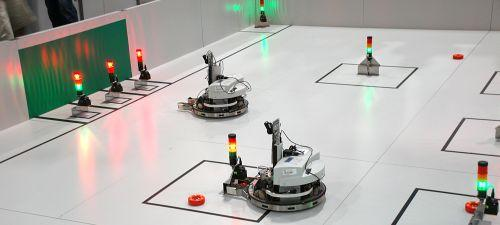
\includegraphics[scale=0.7]{pics/llsf1}
\label{Figure 1}
\caption{A half of the LLSF field.  \textcolor{red}{refferenz schrecklich~\cite{LLSFGermanOpen} Own Picture????}}
\end{figure}
Figure 1 shows this hall and the basic elements. The Robots are Robotinos by Festo~\cite{Robotino}. They hold omni-directional wheels, a showel to move pucks and other sensors added by the participants. The orange pucks represent resouces and products. They are equiped with a RFID-chip which stores the type of the puck. The lamps on the field are the machines. They use RFID to convert recourses into producs and trash. There are different types of machines. They can produce different product-types, produce intermediate products, recycle trash or are used for delivery. The traffic-light on top of the machines indicates the machine-status. Beside these visual elements there is also a refbox which automatically communicates with the robots during the game. The refbox provides the current phase and tasks of the game.
\subsection{Fawkes}
Fawkes is an open source robot software framework developed by the Knowledge-basede Systems Group~\footnote{\url{www.kbsg.rwth-aachen.de/}} at RWTH Aachen University. It is written for Linux and follows a component-based software design~\cite{FawkesDesign}. It provides an infrastructure to load and unload binary components, implemented as plugins, at runtime and a blackboard for communication between the plugins. A plugin can access the blackboard via interfaces. Because of this design, Fawkes is very flexible and dynamic. The interchangeability of the plugins, which is caused by the well defined interfaces, makes hardware abstraction and reuse easy.\\
\subsection{Gazebo}
Gazebo is an open source multi-robot simulator~\cite{GazeboDesign}. It simulates the behavior of robots and other objects physically in a three dimensional world. The open source engine Ogre~\footnote{\url{http://www.ogre3d.org}} is used for the graphical presentation of the simulation. Physics are simulated with the Open Dynamics Engine~\footnote{\url{http://www.ode.org/}}. Gazebo was originally developed for outdoor applications and aims to simulate robots in a complex and realistic environment. Besides the physical simulation, it does this by generating data for different types of sensors. Gazebo can simulate laser range finders, cameras, sonar sensors, bumpers and more. This makes it able to do realistic and low level simulation. A simulation in Gazebo is made by creating robot and world models and developing Gazebo-plugins for behavior. These plugins can control objects in Gazebo and communicate with other software.
\subsection{Proposed Bachelor Thesis}
The primary goal of the proposed bachelor thesis is to develop a multi-robot simulation environment in Fawkes for the LLSF competition with Gazebo. This will speed up and simplify many current and future developments. Particularly robot coordination will be made easier because there the testing with real robots is even more difficult and time consuming. Some of the the current developments are a high level agent for the exploration phase of LLSF, a laser-cluster-detector that locates obstacles with a laser sensor and a map of the environment and a vision detector for different combinations of light signals including blinking lamps. All these can benefit from the simulation. The agent can easily be tested because its behavior is shown visual in realistic simulation \textcolor{red}{By now finished world in Gazebo FIGURE}. The current simulation for the high level agent is only text-based and does not simulate any actions on a lower level (e.g. all movement orders return that they succeeded after a few seconds). The laser-cluster-detector would benefit from the simulation because the laser data generated done by Gazebo is relatively realistic~\footnote{This has to be proven by the thesis, but it is intuitively right because laser sensors are quite accurate and a geometrical calculation by Gazebo is easy.} and it is possible to look at different situations much faster. Even the vision task can benefit from the simulation because the vision plugin can first be made working as a whole with simple images. The neccessary vision tuning can then be done as a second step with a already tested structure it is embedded in. Of course simulation never can completely substitute testing on the real robot, but it saves a lot of time. This has many causes. There is no need to get the real robots running which can take a lot of time in practise. The logic can be tested seperate from real world problems such as inaccuracy or badly synchronized clocks. An other advantage of the simulation is that ever the developers do not work on the same system. So there are no messed up configuration files and less problems with revision controlling. After reaching the primary goal the thesis will continue by making the simulation more general, so that it can be easily configured for different scenarios. an other further goal is to add more features such as communication brakedown or computational evaluation of the working plugins to the simulation.\\
Structural, the multi-robot simulation for LLSF will consist of Fawkes and Gazebo plugins and models for Gazebo. The interchangeability of plugins in Fawkes makes it possible that the simulation only needs to exchange the robot hardware plugins on the lowest level by robot simulation plugins. All plugins on upper levels do not need to be changed and can work in the simulation the same way as in reality. The models for Gazebo will represent all physical objects in the LLSF game (e.g. the Robotino and the Machines). The Gazebo plugins will control the behavior and sensing of all dynamic elements in the game (e.g. the Robotino and the refbox).\\
In the following the proposal will give an overview of the related work in section 2. This section will be divided in the context the thesis will be embedded in, other simulators and other multi-robot simulations. Section 3 will present the proposed work in detail with primary and further goals. Section 4 will give a schedule and in section 5 some methods of afterwards evaluation are proposed. The conclusion is found in section 6.


\section{Related Work}
\subsection{Existing Context}
The work of the proposed thesis is embedded in a already existing context of work. The Carologistics team~\footnote{\url{http://trac.fawkesrobotics.org/wiki/Carologistics}} participates in LLFS and is a joint team consisting of Knowledge-based Systems Group at RWTH Aachen University, IMA/ZLW \& IFU Institute Cluster at RWTH Aachen University and Department for Electrical Engineering and Information Technology, Robotics Group at FH Aachen. The team has developed a working system for LLSF and participated in the RoboCup 2012 in Mexico. Thus, there are many things to do. There are changes in the rules and challenges of LLSF. Furthermore the team is changing the architecture of the Robotinos. A laptop mounted on the robot should ensure that there is enough computational power (e.g. for localization). Of course, the most general task is to improve the performance of the robot to be successful in the competition. The work of Carologistics is based on fawkes. It additionally uses ROS~\footnote{\url{www.ros.org/}} for \textcolor{red}{what?}.\\
Some work was already done on Gazebo for Fawkes. Bastian Klingen developed in his diploma thesis~\cite{KlingenDA} a scene reconstruction for fault analysis. It was primary made for a mobile robot which has to pick up a colored cup with a gripper arm. The motions, sensor data and belief of the robot are stored in a database. If the process fails, the scene reconstruction visualizes what happened from the robots point of view to make fault analysis possible. The visualization was made with Gazebo. In the implementation Klingen also made a general Gazebo-aspect for Fawkes. This can be used as a starting point for the proposes thesis and may be enchanted if it is necessary or useful \textcolor{red}{details???}.
\subsection{Comparison of Simulators}
This subsection presents an overview of the mainly used robot simulators that are able to support LLSF. Afterwards there is reasoned why Gazebo is chosen as the most appropriate simulator for the thesis.
\subsubsection{Other Robot Simulators}
A often used robot simulator is \textit{Stage}~\footnote{\url{playerstage.sourceforge.net/index.php?src=stage}}. It is part of the \textit{Player/Stage} project~\cite{PlayerStage} and provides an easy to use simulation environment for \textit{Player}, a widely used robot control interface. Stage is an open source 2D-simulator and supports large populations of robots.\\
\textit{Robotino Sim Professional}~\footnote{\url{http://www.festo-didactic.com/int-en/learning-systems/software-e-learning/robotino-sim-view/robotino-sim-professional.htm}} is a 3D-simulator for the Robotino developed by it's manufacturer Festo. Is is a commercial software and only usable in Microsoft Windows.\\
\textit{Webbots}~\footnote{\url{www.cyberbotics.com}} is a commercial 3D-simulator~\cite{Webbots}. It is platform independent and can simulate several robots at the same time. It is able to run simulations faster then real time if the complexity of the simulation allows this.\\
\textit{USARSim}~\cite{USARSim} was originally intended as a urban search and rescue simulation but it can also be used for other domains. It is platform independent and free of charge for research and education. It is used in the Rescue Virtual Robot Competition within the RoboCup.\\
\textit{SIMRobot}~\footnote{\url{www.informatik.uni-bremen.de/simrobot}} is an open source 3D-simulator and platform independent. It is used by multiple teams in the RoboCup~\cite{SIMRobot}. It has been developed by the University Bremen since 1994.\\
The \textit{Microsoft Robotics Developer Studio}~\footnote{\url{www.microsoft.com/robotics}} is free for noncommercial use and bound to Microsoft Windows. Besides the simulation it offers standartization for robotic control and several tools for robot development~\cite{MicrosoftRoboticsStudio}.
\subsubsection{Advantages of the Gazebo Simulator}
The Gazebo simulator has many advantages for this thesis~\cite{GazeboDesign}. It is open source what makes it free to use and easy to edit if something is missing. For example drawing additional lines during runtime is not supported. \cite{KlingenDA} implemented this to draw a grid. It is important that Gazebo is a 3D-simulator because camera sensors can not be simulated in a two dimensional simulator. The physics engine and realistic graphics are indispensable for a realistic simulation. It is possible in Gazebo to assign for example friction and reflection values to an object. So, even the problem of a reflecting ground can be simulated if you are developing a light-seeking vision program. Other advantages are that Gazebo runs in Linux and has an active community and a beginner friendly documentation. Furthermore, it already includes many common used robots-models and sensors. Therefore it is only rarely necessary to implement own sensor plugins. Additional to that, Gazebo seems to be well suited for future work. It is a general multi-robot simulator and is well founded. Gazebo was chosen as the basis for the \textit{DARPA Robotics Challenge Simulator 2013}~\footnote{http://spectrum.ieee.org/automaton/robotics/robotics-software/darpa-robotics-challenge-simulation-software-open-source-robotics-foundation}. A more practical advantage of Gazebo is that some work was already done on Gazebo in Fawkes by~\cite{KlingenDA}.\\
There are not many disadvantages of Gazebo. One is that Gazebo can not handle a larger number of robots~\cite{GazeboDesign}. The complexity of the simulations limits the number of robots on the order of ten~\footnote{Information from 2004}. This is no problem for this work because in LLSF there are only three robots.
\subsection{Other Multi-Robot Simulations}
There are several other multi-robot simulation environments. \cite{MultiLevelAbstraction}~simulates the Middle-size soccer league of RoboCup and also works with Gazebo, but used Player for robot control. In the Middle-size soccer league there are two teams with five robots under the size of 90 cm. Therefore the simulation has to handle up to ten robots at once. In this work similar equipment was simulated as used by Carologistics. \cite{MultiLevelAbstraction}~simulated a prototype of omni-directional wheels and an omni-vision camera. Figure 2 shows these two devices in the simulation.
\begin{figure}
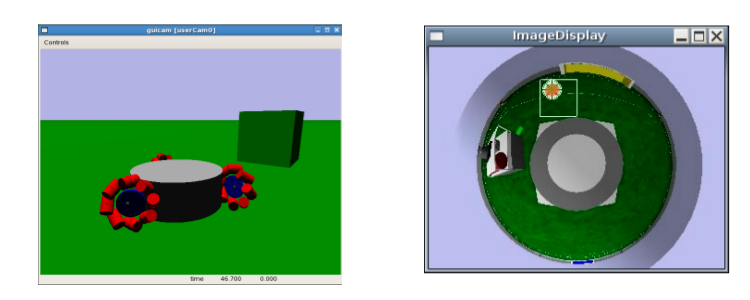
\includegraphics[scale=0.5]{pics/GazeboEquipment}
\label{Figure 2}
\caption{An omni-directional wheel prototype build in Gazebo (left) and the simulated picture taken of an omni-vision camera (right)~\cite{MultiLevelAbstraction}.}
\end{figure}
The omni-directional wheels of the Robotino work in the same way, but have a different design that needs to be modeled. The omni-vision camera mounted on the Robotino of Carologistics is very similar to the camera on the soccer-robots. The gazebo-plugin for this camera can be reused. The main point of~\cite{MultiLevelAbstraction} is the multi-level abstraction of the simulation. That means that the simulation is able to simulate with different complexities. For example, the simulation can simulate on the physical level, where the robot software has to do movements and sensing as in the real world, and on a high logical level, where the robot moves exactly like intended and the simulation tells the robot exactly where it is located. These different abstraction levels are also important for the proposed thesis because they make the simulation more flexible and are well suited as milestones of the development of the simulation. \cite{MultiLevelAbstraction}~also shows that the speed of the simulation is an important aspect. If the simulation does not run fast enough to simulate in real-time, the behavior of the simulated robots can change because many processes running on the agent measure the time itself. \cite{MultiLevelAbstraction}~dealed with this problem by changing the source code of the robot-software and telling it the simulation time instead of the system time. If possible, this should be avoided by the thesis.\\
An other related work is~\cite{SurveillanceSystem}. It used Gazebo and Player to simulate a surveillance system with Pioneer3AT robots. In this system several robots have to monitor an outdoor area and find possible intruders. Therefore the robots have to spread over the area and coordinate their movements. The simulation was important for the development of the system because it could quickly simulate different areas and situations.

\section{Details of Work}
This section presents the goals of the thesis and how they will be reached in detail. Because it is difficult to estimate how much time the development of the simulation will take and what difficulties will appear during this time, we define the minimum goals here and give some additional goals, which will be worked on if there is some time left. These additional goals are separated in wanted goals and optional, but very attractive goals. Table 1 shows an overview of the goals and their level.

\begin{table}
\begin{tabular}{|r||p{10cm}|}
\hline
Minimum & \begin{itemize}
\item Simulation environment for LLSF
\item High level simulation of the Robotino (exact position, exact movement)
\item Multiple communicating robots at the same time
\item Measurement of simulation speed and qualitative evaluation of the simulation
\item Detailed documentation how to use the simulation in the wiki
\end{itemize}\\ \hline
Wanted & \begin{itemize}
\item More general simulation (with abstraction layer)
\item Low level simulation of the Robotino (motor movement, laser and camera sensors)
\item Quantitative evaluation of simulation
\item Evaluation of robot behavior in simulation in comparison to reality
\item Detailed documentation how to extend the simulation for other tasks
\end{itemize}\\ \hline
Maximum & \begin{itemize}
\item Simulation with multi-level abstraction
\item Performance measuring of LLSF playing robots (automated running of the simulation)
\item Speedup of the simulation (if possible)
\item Simulation of LLSF challenges
\item Use of simulation at other tasks
\end{itemize}\\
\hline
\end{tabular}
\label{Table 1}
\caption{Minimal, wanted and maximal goals, which should be reached by the thesis.}
\end{table}
The goals are designed and ordered this way so that the minimal goals can be achieved first. The other goals depends on the ones before. This is especially important for the abstraction of the simulation environment and the detail-level of the simulation. First a simple, working and quickly achievable simulation for LLSF with exact motion and position sensing should be developed. With this basis, further work is possible.\\


\section{Timetable}
\section{Evaluation}
\section{Conclusion}

\bibliographystyle{plain}
\bibliography{references}

\end{document}
